\documentclass[a4paper]{article}
\usepackage{graphicx}
\begin{document}
\begin{figure}
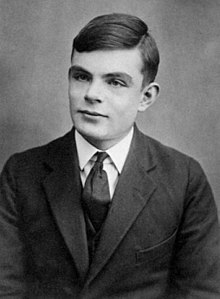
\includegraphics[width=10cm]{Turing.jpg}
\caption{Turing machines are named after Alan Turing}
\label{figure:turing}
\end{figure}

Alan Mathison Turing\ref{figure:turing}(23 June 1912 – 7 June 1954) was an English mathematician, computer scientist, logician, cryptanalyst, philosopher, and theoretical biologist. Turing was highly influential in the development of theoretical computer science, providing a formalisation of the concepts of algorithm and computation with the Turing machine, which can be considered a model of a general-purpose computer.He is widely considered to be the father of theoretical computer science and artificial intelligence.

Turing machines are the simplest and most widely used theoretical models of computing. Far too slow and unwieldy ever to be embodied in a real device, these conceptual machines nevertheless seem to capture everything we mean by the term \textit{computation}. Not only do Turing machines occupy the top level of the Chomsky hierarchy, but they also seem capable of computing any function which is computable by any other conceptual scheme.

\section{Alan Turing}
The Turing machines described in section are named after Alan Turing.

You can find Turing's publications in Google scholar. \cite{googlescholar}
His paper on the Entscheidungsproblem was published in 1937. \cite{alanturing}
He wrote about thinking machines in 1950. \cite{turingomnibus}
\bibliographystyle{unsrt}
\bibliography{turing}

\end{document}

